\chapter{Introduzione}

La Blockchain è uno degli argomenti più caldi nell'industria dell'IT. In questo
capitolo cercheremo di fare chiarezza, partendo dalle origini di questa tecnologia
sino ad arrivare allo stato dell'arte odierno.

\section{DLT}
Per capire cosa è una \textbf{Distribuited Ledger Technology} (DLT) è necessario
innanzitutto chiarire il concetto di Ledger.

Un \textbf{Ledger}, parola che in italiano traduciamo come \textit{Libro Mastro},
è il registro principale in cui sono riunite tutte le transazioni economiche
che compongono un dato sistema contabile. In sostanza si tratta di un documento
nel quale vengono registrate tutte le transazioni economiche, dove viene
indicata la data della transazione, la cifra scambiata e i soggetti coinvolti
nella transazione (chi dà e chi riceve). Le modifiche apportate possono essere solo
di tipo incrementale: non si possono apportare modifiche o cancellare record,
ma solo aggiungere nuove righe al ledger.

Poiché di fatto contiene tutta la storia del sistema contabile, il legder è anche
lo strumento da consultare quando si vuole stabilire quanto denaro possiede un certo
individuo, e se quindi può effettuare un pagamento oppure no per insufficienza
di fondi.

Il Ledger è uno strumento che da secoli viene usato dall'uomo. Le implementazioni
classiche si basano su un soggetto fidato, come ad esempio una banca, che è
l'unico ad essere autorizzato ad apportare modifiche. In questo modo è




\section{Blockchain}
La \textbf{Blockchain} non è altro che una tipologia di DLT. Spesso nell'linguaggio
comune queste due parole vengono usate come sinonimi, ma in questa tesi ci impegneremo
nel mantenere questa distinzione.

Una Blockchain è una catena di transazioni in continua crescita. Le transazioni sono
raggruppate in blocchi che sono collegati tra di loro con tecniche
crittografiche.

Ogni blocco è composto da:
\begin{itemize}
	\item L'hash crittografico del blocco precedente
	\item Un timestamp, ossia la data e l'ora dell'aggiunta del blocco alla catena
	\item Un insieme di transazioni
\end{itemize}
La Blockchain è stata inventata da Satoshi Nagamoto nel 2008 per essere utilizzata
come ledger pubblico per la gestione della criptovaluta Bitcoin. ,
grazie all'utilizzo della blockchain, è stato possibile risolvere il problema
del \textit{double-spending} senza ricorrere ad una autorità fidata.


\section{Smart Contracts}
Lo Smart Contract è uno strumento che ha un forte legame con la blockchain e che ha un ruolo chiave
nelle applicazioni enterprise e non solo.
Ciò nonostante, non vi è ancora un chiaro consenso sulla definizione di Smart Contract.

L'idea di Smart Contract risale a ben prima della nascita della Blockchain. È stata infatti introdotta
per la prima volta nel 1994 da Nick Szabo, per poi
essere formalizzato da lui stesso nel 1997 \cite{szabo-smart-contracts}.
Secondo la definizione originale,
\begingroup
\advance\leftmargini 2em
\begin{quote}
	{\bf
		{\em Smart contracts combine protocols with user interfaces to formalize
			and secure relationships over computer networks.
			Objectives and principles for the design of these systems
			are derived from legal principles, economic theory,
			and theories of reliable and secure protocols.}
	}
\end{quote}
\endgroup

Più recentemente sono emerse definizioni in linea con la realtà contemporanea.
In \cite{making-sense-of-bsc}, Stark fornisce una panoramica dei due diversi significati che il termine
Smart Contract ha assunto:
\begin{enumerate}
	\item \textbf{Smart Contract Code}: opera nel mondo naturale,
	      coinvolgendo l'uso di agenti software che tipicamente,
	      ma non necessariamente, operano su un ledger condiviso. La parola contratto in questo senso
	      indica che gli agenti software devono sottostare ad alcuni vincoli e possono prendere il controllo
	      di alcuni asset in un ledger condiviso. Non vi è un chiaro consenso  There is no clear consensus on the
	      definition of this use of the term “smart contract” — each definition is different in subtle
	      ways [18, 17, 16, 3]. Stark renames these agents as smart contract code.
	\item \textbf{Smart Legal Contract}: The second focuses on how legal contracts can be expressed and executed in software.
	      This therefore encompasses operational aspects, issues relating to how legal contracts
	      are written and how the legal prose should be interpreted. There are several ideas and
	      projects which focus on these aspects such as the Ricardian Contract [7], CommonAccord
		      [4] and Legalese [13]. Stark renames these as smart legal contracts.
\end{enumerate}
Partendo dall'analisi di Spark, Clack et al. in \cite{Clack2016SmartCT} propongono una definizione
di più alto livello che include entrambi i significati di cui sopra, basata sui temi
dell'automazione e dell'applicabilità:
\begingroup
\advance\leftmargini 2em
\begin{quote}
	{\bf
		{\em A smart contract is an automatable and enforceable agreement. Automatable by computer,
			although some parts may require human input and control. Enforceable either by legal
			enforcement of rights and obligations or via tamper-proof execution of computer code.  }
	}
\end{quote}
\endgroup
\begingroup
\advance\leftmargini 2em
\begin{quote}
	{
		{\em Uno smart contract è un accordo automatizzabile e applicabile. Automatizzabile da computer,
				sebbene alcune parti possano richiedere input e controllo umani. Applicabile sia attraverso
				l'obbligatorietà legale di diritti e doveri o tramite
				l'esecuzione di codice informatico a prova di manomissione.}
	}
\end{quote}
\endgroup
Questa definizione è sufficientemente astratta da includere sia lo "smart legal contract"
(dove l'accordo è un accordo legale, che è in grado di essere eseguito automaticamente da un software)
e lo "smart contract code" (che potrebbe non essere necessariamente legato ad un accordo legale formale,
ma che comunque viene eseguito automaticamente).



\section{Vulnerabilità negli Smart Contract}
Come abbiamo visto gli Smart Contract permettono l'esecuzione di codice arbitrario
sulle blockchain, permettendo interazioni automatizzate tra diversi attori in un contesto
\textit{trustless} senza ricorrere all'utilizzo di terze parti fidate.

Gli Smart Contract si ritrovano a gestire diversi miliardi di USD in criptomoneta,
attirando quindi le attenzioni di malintenzionati. In questa sezione analizzeremo
diverse vulnerabilità emerse nel corso del tempo e mostreremo
alcuni strumenti in grado di aiutarci nello sviluppo di Smart Contract sicuri.

\subsection{Classificazione delle vulnerabilità}
Secondo Nikolic et al. \cite{Nikolic2018FindingTG},
gli Smart Contract vulnerabili possono essere divisi in tre categorie.

\paragraph{Prodigal Contracts}
Esistono alcune categorie di destinatari tipici delle transazioni effettuate
dagli smart contracts. I contratti spesso restituiscono fondi ai
proprietari, agli indirizzi che hanno inviato
criptomoneta ad essi in passato (ad es. nelle lotterie) o a indirizzi
per i quali vi è una ragione specifica (ad es. invio di una ricompensa).
I \textbf{prodigal contracts} sono contratti che inviano fondi ad
indirizzi arbitrari che non rientrano nelle categorie di cui sopra.

\paragraph{Suicidal Contracts}
I contratti spesso hanno una opzione di sicurezza che permette al proprietario
o a un account fidato di uccidere il contratto in situazioni di emergenza,
come un attacco o un malfunzionamento. Se questa funzionalità non è correttamente gestita
un contratto potrebbe essere ucciso da un qualunque account arbitrario.
Se è così, allora il contratto rientra nella categoria dei \textbf{suicidal contracts}.

\paragraph{Greedy Contracts}
I \textbf{greedy contracts} sono i contratti che rimangono vivi e detengono
criptomoneta per un tempo indefinito e che non permettono il riscatto dei
fondi contenuti in alcuna circostanza.

\subsection{Come costruire Smart Contracts sicuri}
Una buona pratica da seguire per sviluppare Smart Contracts sicuri è
informarsi sulle vulnerabilità note.
Lo Smart Contract Weakness Classification Registry \cite{swc-registry} fornisce un elenco
costantemente aggiornato catalogo di vulnerabilità e anti-pattern noti insieme ad esempi
di casi reali.

\subsubsection{Strumenti per l'individuazione di vulnerabilità}
Esistono diversi strumenti in grado di rilevare eventuali vulnerabilità presenti
negli Smart Contracts.  Ne proponiamo un paio tra quelli che operano con
gli Smart Contract di Ethereum.

\paragraph{SECURIFY} Tool: \cite{secufiry-url}. Paper: \cite{secufiry-paper}.
Si tratta di uno strumento per l'analisi statica di Smart Contract scritti in Solidity. È in grado
di dimostrare che i comportamenti degli Smart Contract sono sicuri/non sicuri
rispetto a determinate proprietà.
L'analisi di Securify consiste in due passaggi.
Per prima cosa analizza simbolicamente il grafo delle dipendenze
del contratto per estrarre informazioni semantiche dal codice.
Quindi usa modelli di conformità e violazione
in grado di individuare condizioni sufficienti per dimostrare se una
proprietà è valida o meno.

\paragraph{MAIAN} Tool: \cite{maian-url}. Paper: \cite{Nikolic2018FindingTG}
È uno strumento di analisi in grado di individuare vulnerabilità direttamente
dal bytecode di Ethereum Smart Contract, senza l'uso dei sorgenti.
Si basa sullo studio delle \textit{trace properties}, impiegando l'uso di
analisi simbolica inter-procedurale e di un validatore.


\section{Stellar}

\textbf{Stellar} è un protocollo decentralizzato ed
open source nato con lo scopo di poter
trasferire denaro attraverso diversi
paesi con costi di transazione irrisori. Il nome della criptovaluta scambiata
è Lumen (\textbf{XLM}).

È stato creato nel 2014 da \textbf{Jed McCaleb} e \textbf{Joyce Kim}.
Si tratta di un progetto fortemente ispirato da \textit{Ripple} (di cui Jed McCaleb
è co-fondatore). A differenza di quest'ultimo, Stellar si pone come obietivo
il facilitare lo scambio di denaro tra privati invece che tra banche.

[...]


\subsection{Gli Smart Contracts in Stellar}
\label{subsec:stellar smart contracts}
% In Stellar gli Smart Contracts di Szabo sono implementati
% attraverso gli Stellar Smart Contracts.

Secondo la documentazione ufficiale \cite{stellar-doc-sc},
uno \textbf{Stellar Smart Contract} (SSC) è espresso come la composizione
di transazioni connesse fra loro ed eseguite secondo certi vincoli.
I vincoli che si possono utilizzare nella realizzazione di SSCs sono:

\begin{itemize}
	\item \textit{Multisignature (multifirma)} - Quali chiavi sono necessarie
	      per autorizzare
	      una certa transazione? Quali soggetti devono concordare in una certa
	      circorstanza affinche si possano eseguire i passi?
\end{itemize}
La Multisignature è il concetto di richiedere firme di soggetti diversi per
effettuare transazioni provenienti da un certo account.
Attraverso pesi e soglie di firma,
viene creata la rappresentazione del potere nelle firme.

\begin{itemize}
	\item \textit{Batching/Atomicity (batching/atomicità)} -
	      Quali operazioni devono avvenire
	      o tutte insieme o fallire?
	      Cosa deve accadere per forzare il successo o il fallimento?
\end{itemize}
Il Batching è il concetto dell'includere più operazioni in un'unica transazione.
L'atomicità è la garanzia che, data una serie di operazioni raggruppate in
un'unica transazione,
al momento dell'invio sul network se anche una sola operazione dovesse fallire,
tutte le operazioni nella transazione fallirebbero.

\begin{itemize}
	\item \textit{Sequence (sequenza)} -
	      In che ordine deve essere elaborata una serie di transazioni?
	      Quali sono le limitazioni e le dipendenze?
\end{itemize}
Il concetto di sequenza è rappresentato sullo Stellar network attraverso
il numero di sequenza. Utilizzando i numeri di sequenza
nella manipolazione delle transazioni è possibile garantire che
transazioni specifiche non possano essere eseguite
nel momento in cui venisse inoltrata una transazione alternativa.

\begin{itemize}
	\item \textit{Time Bounds (limiti temporali)} -
	      Quando è possibile elaborare una transazione?
\end{itemize}
I limiti di tempo sono vincoli sul periodo di tempo durante il quale
una transazione è valida. L'utilizzo dei limiti di tempo
consente di rappresentare i periodi di tempo in un SSC.

\section{L'adozione della blockchain nelle industrie}
Il successo o il fallimento di uan tecnologia è molto spesso legato più ... che alla bontà della tecnologia stessa.
In questa sezione vedremo alcuni dati e statistiche che ci aiuteranno a capire quale è
lo stato dell'arte per quanto riguarda l'adozione delle tecnologie blockchain nelle industrie
e cosa aspettarci per il futuro.

\subsection{Il panorama attuale}
\begin{figure}[H]
	\centering
	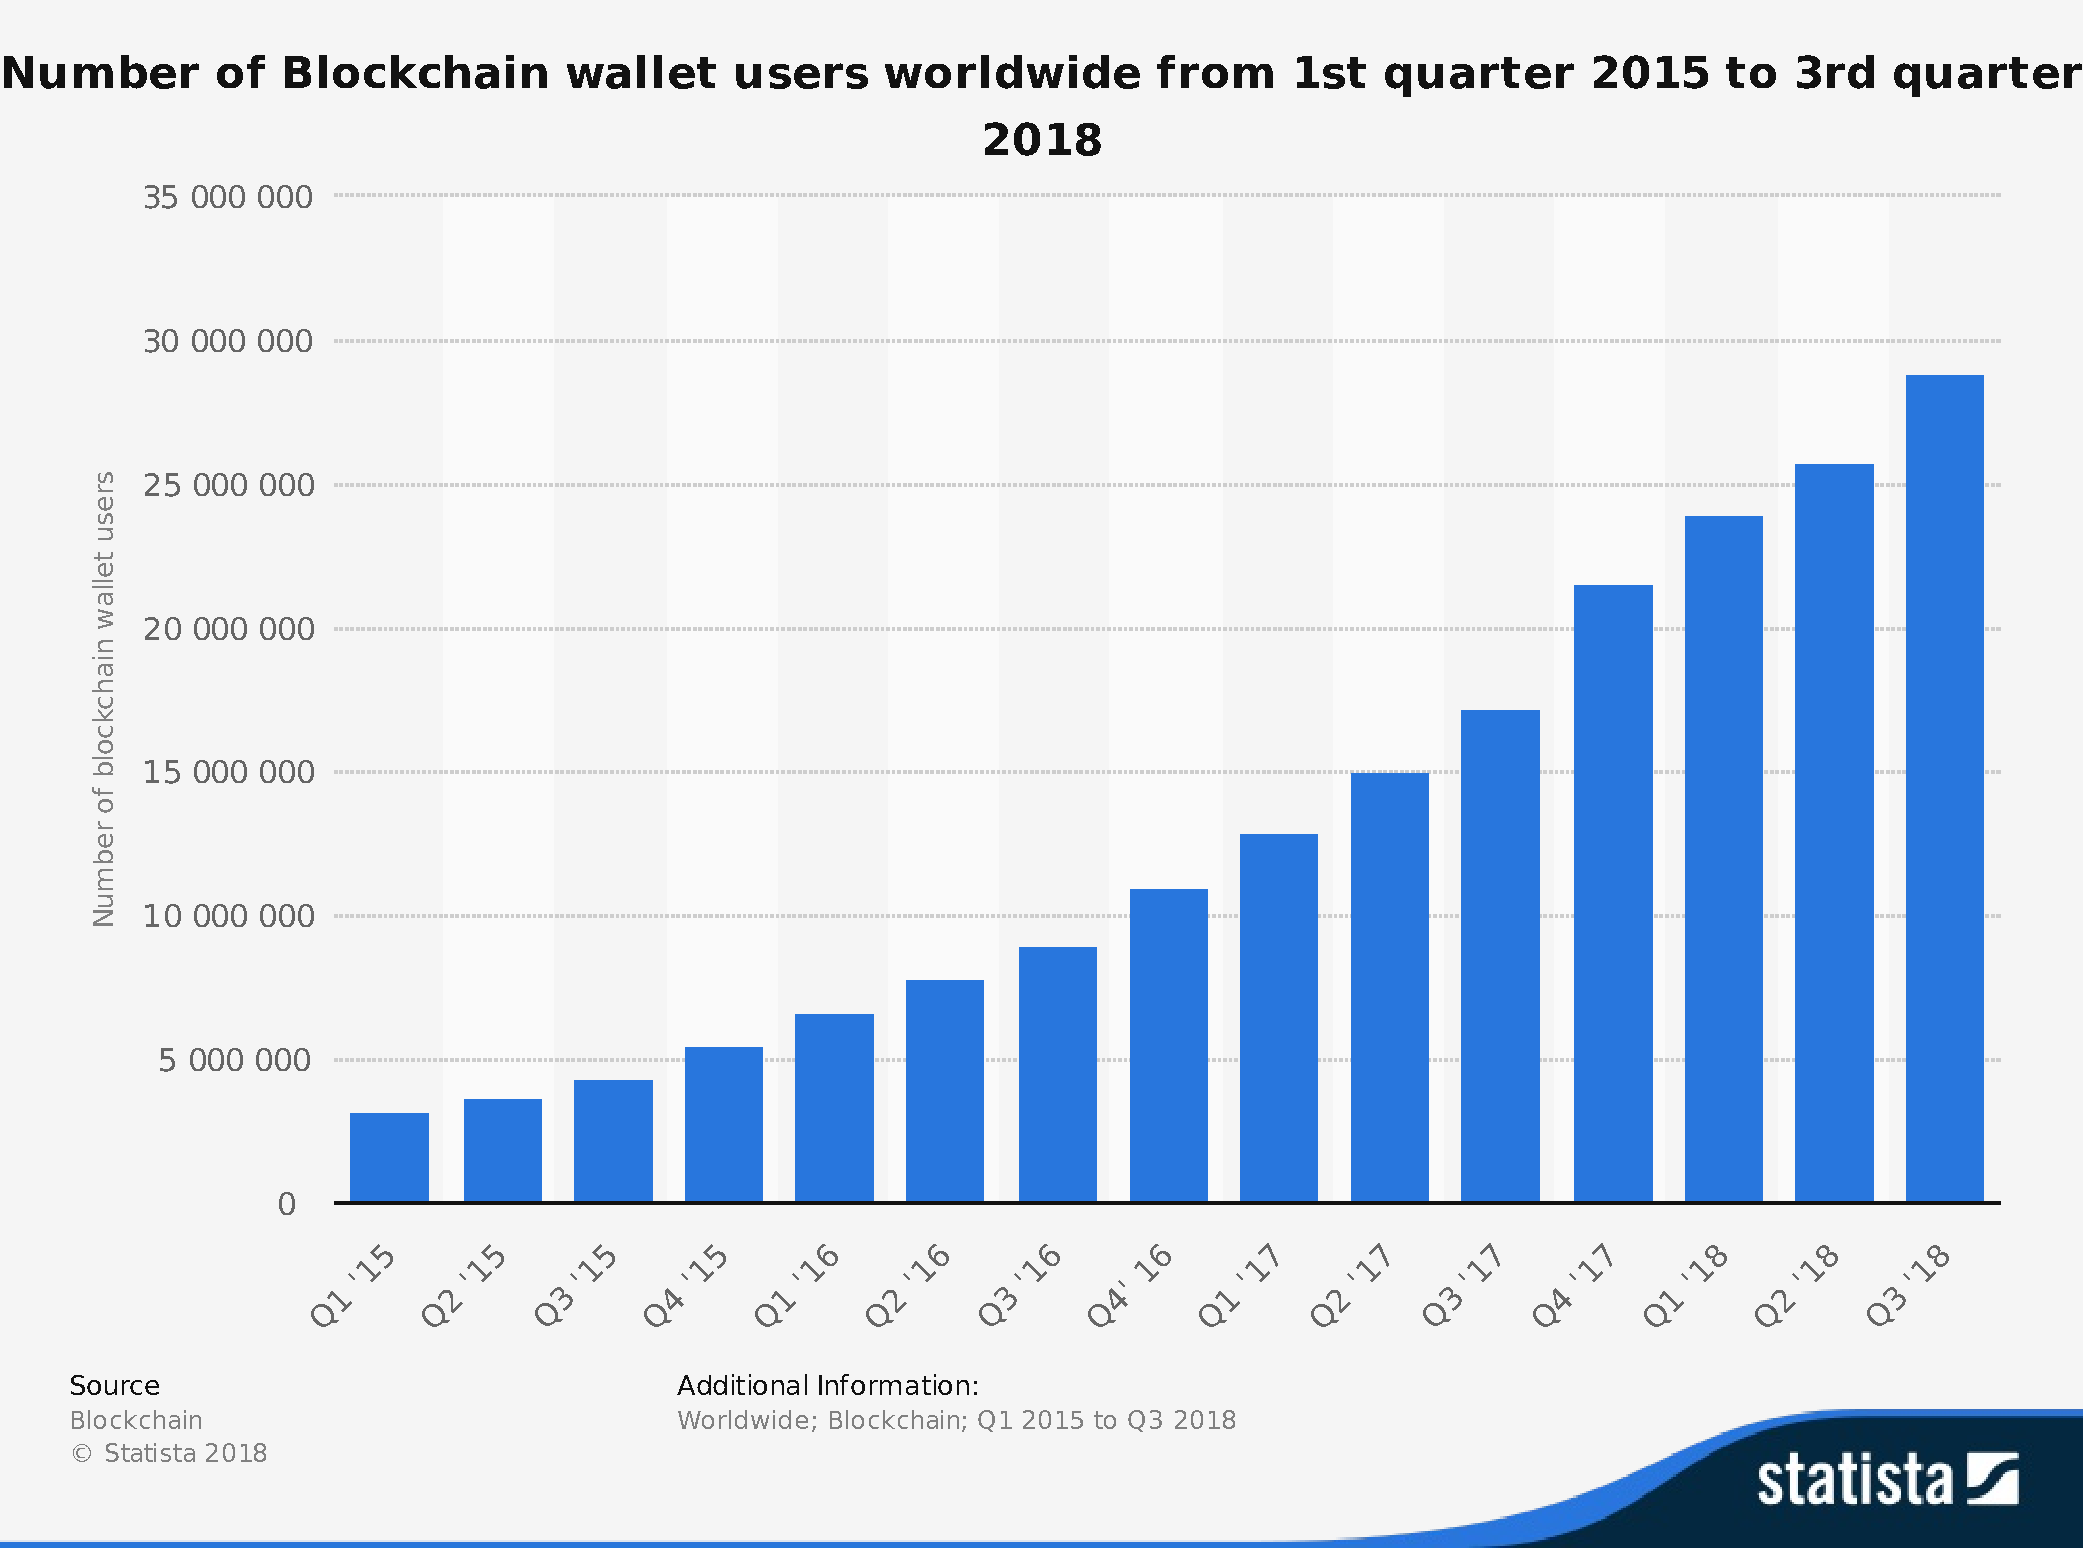
\includegraphics[width=.75\linewidth]{images/chap_intro/number-of-blockchain-wallet.pdf}
	\caption{Numero di portafogli blockchain nel mondo \cite{number-of-blockchain-wallet}}
\end{figure}
\begin{figure}[H]
	\centering
	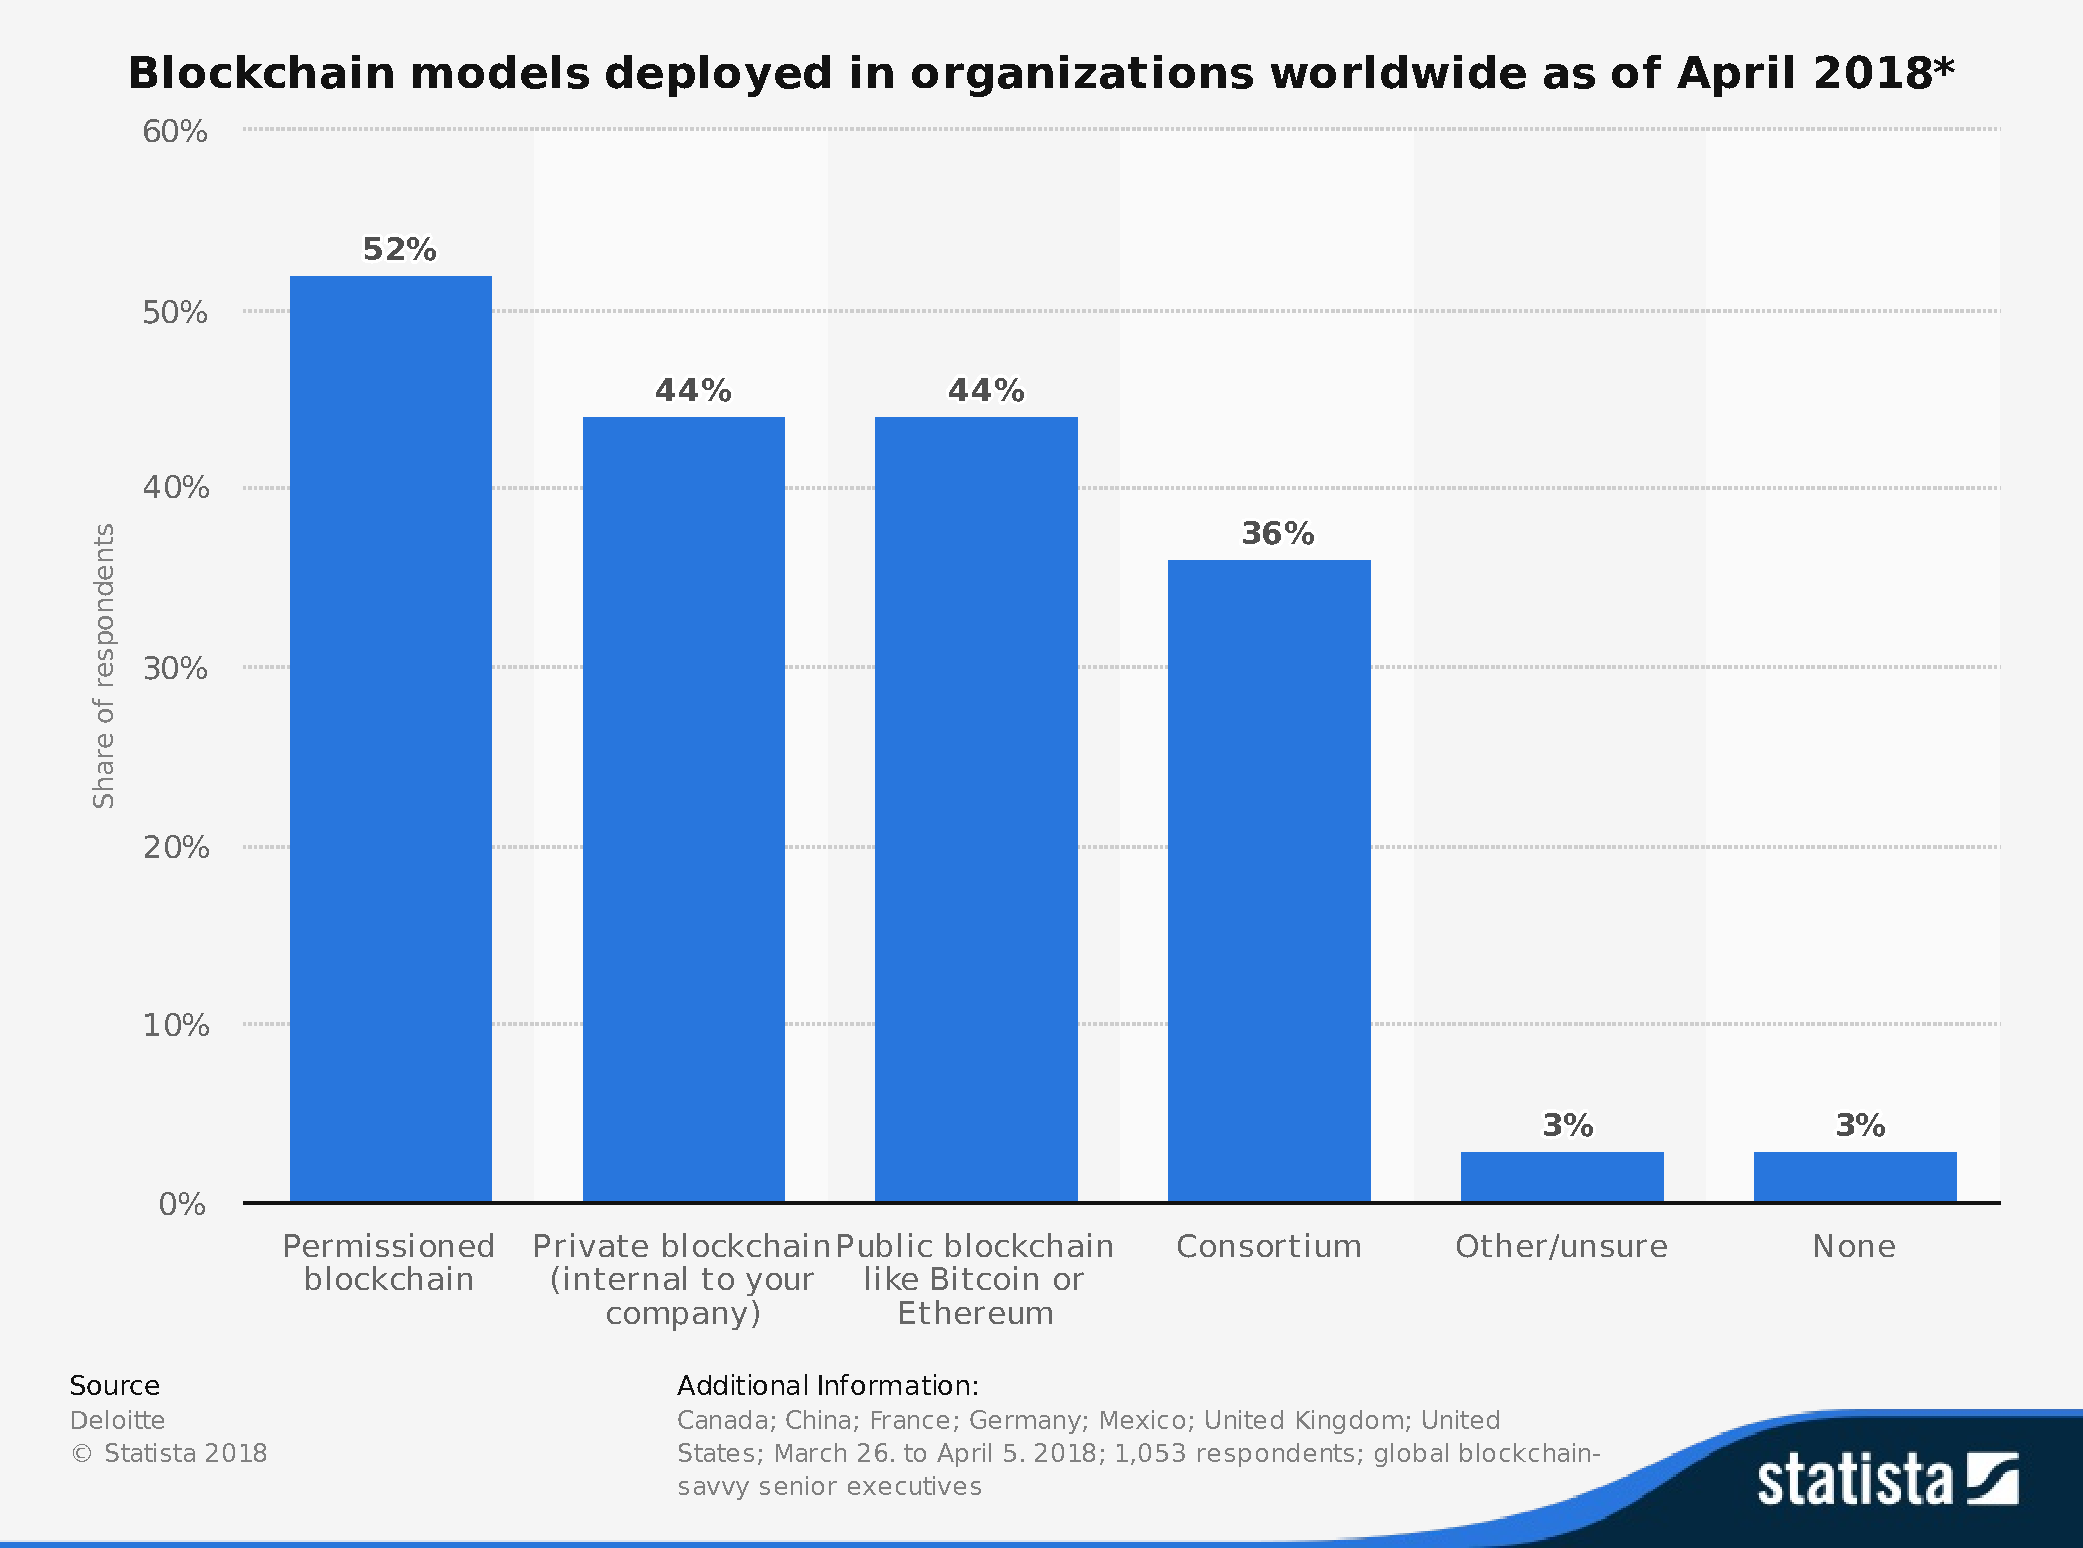
\includegraphics[width=.75\linewidth]{images/chap_intro/model-focus-for-blockchain.pdf}
	\caption{Modelli blockchain utilizzati dalla organizzazioni \cite{model-focus-for-blockchain}}
\end{figure}

\begin{figure}[H]
	\begin{minipage}{0.48\textwidth}
		\centering
		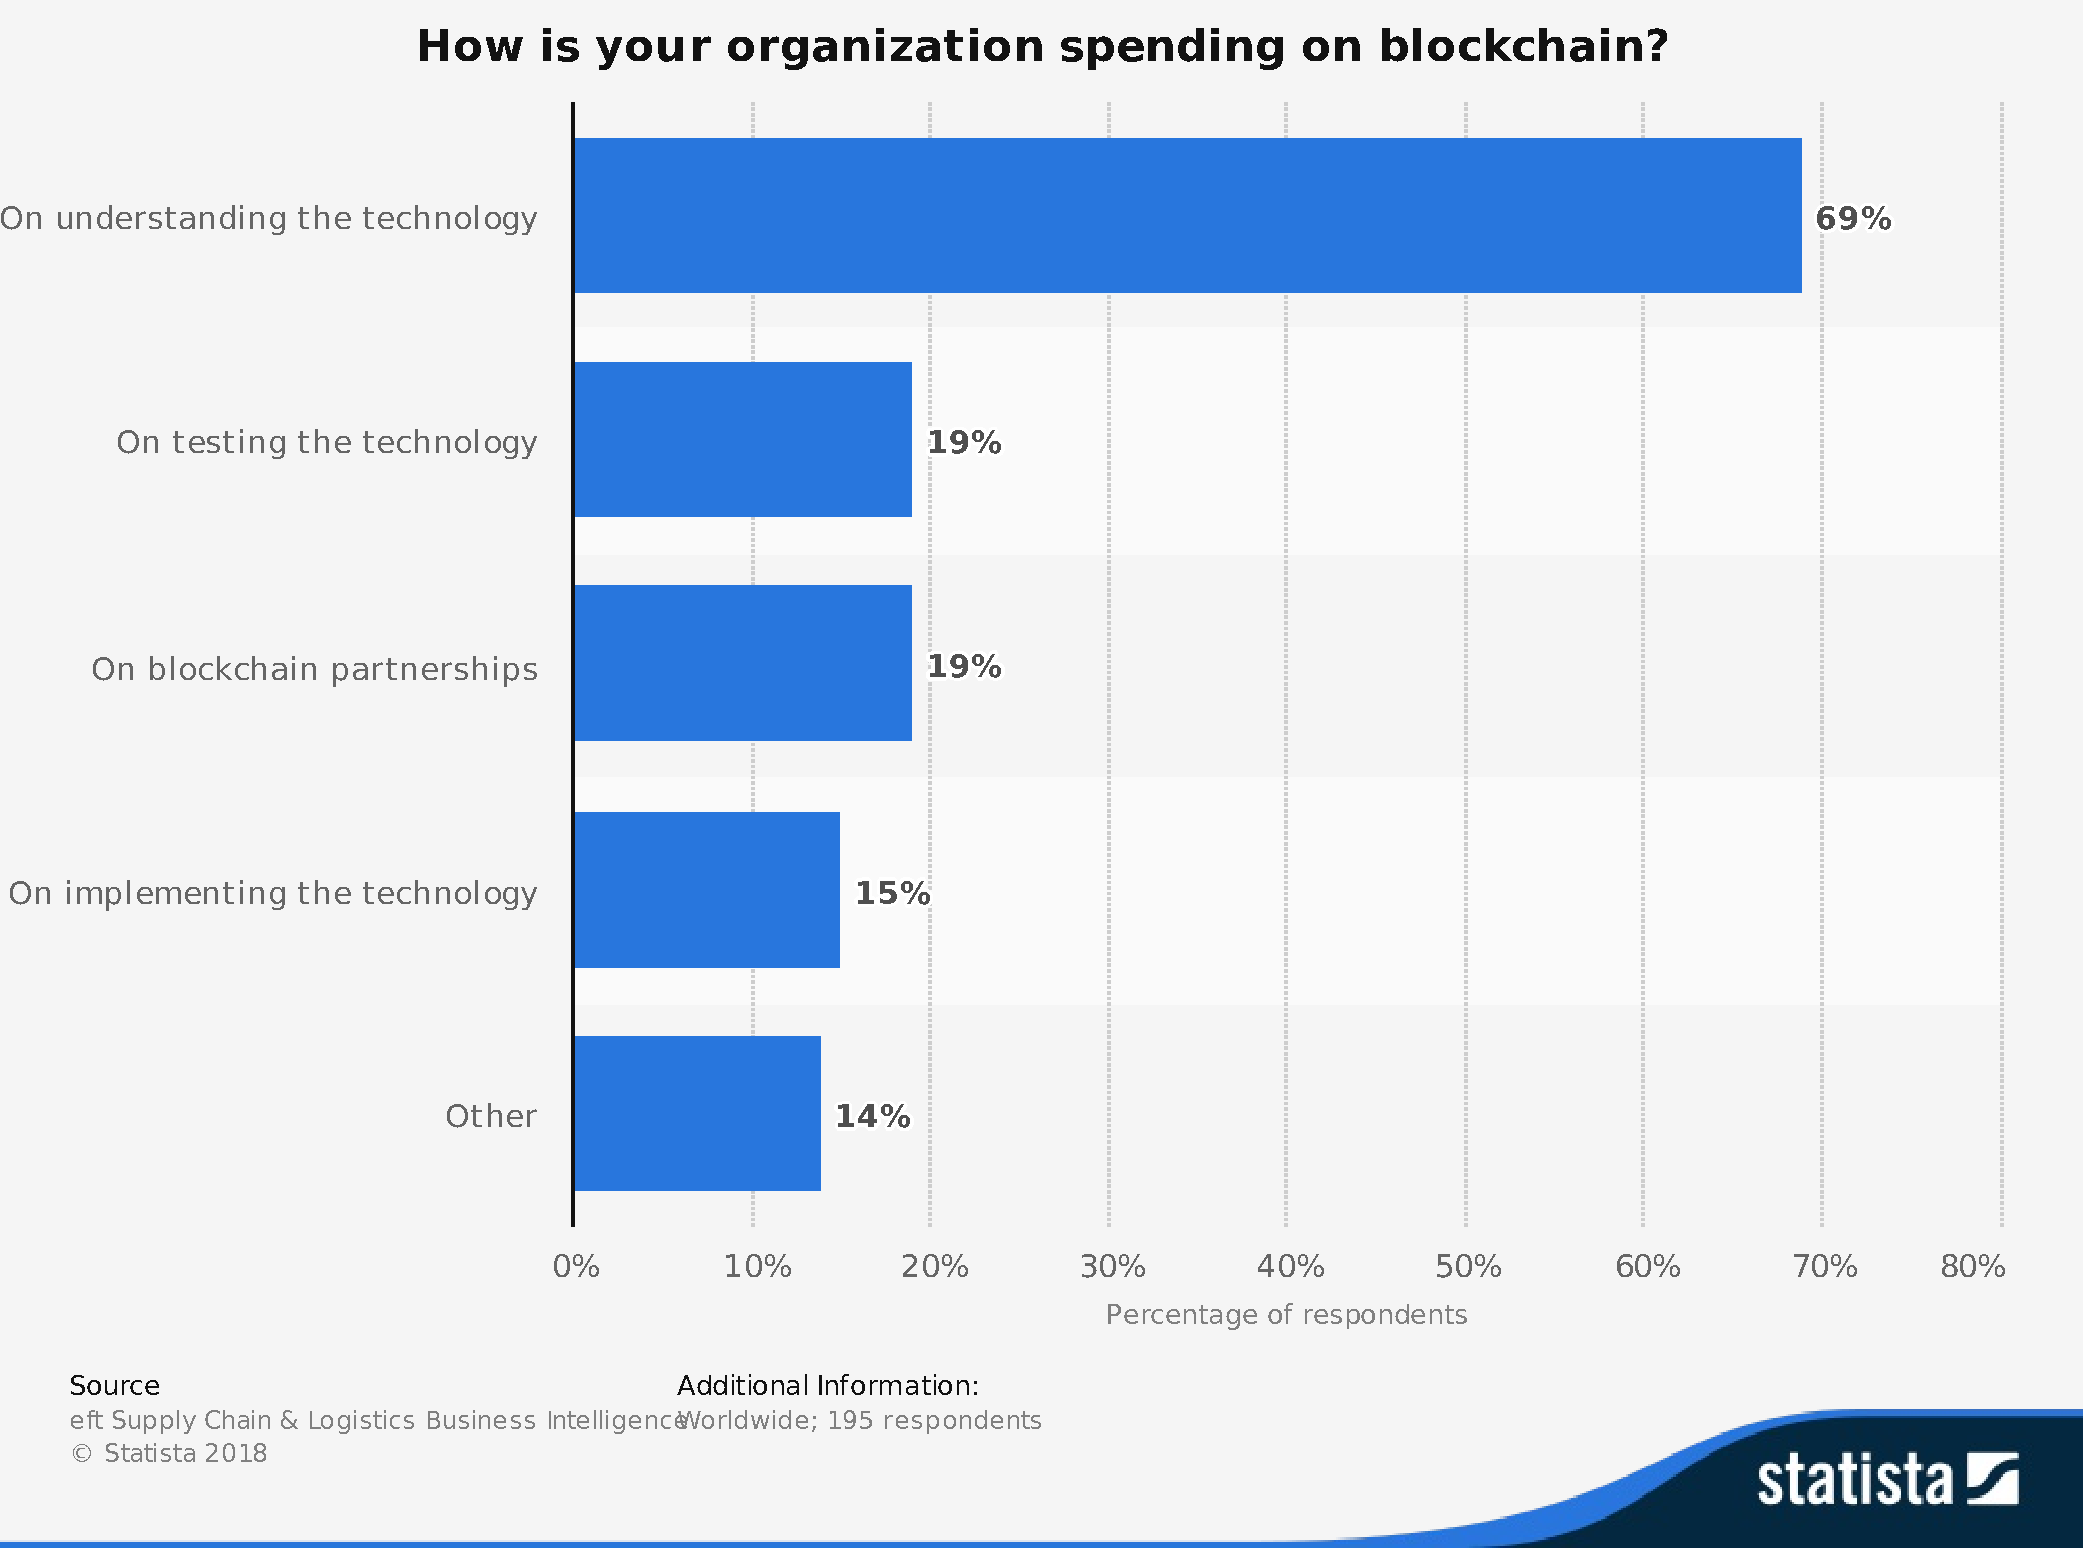
\includegraphics[width=1\linewidth]{images/chap_intro/top-spending-in-supply-chain-industry.pdf}
		\caption{Sondaggio: in che modo la tua organizzazione sta investendo nella blockchain?
			\cite{top-spending-in-supply-chain-industry}}
	\end{minipage}\hfill
	\begin{minipage}{0.48\textwidth}
		\centering
		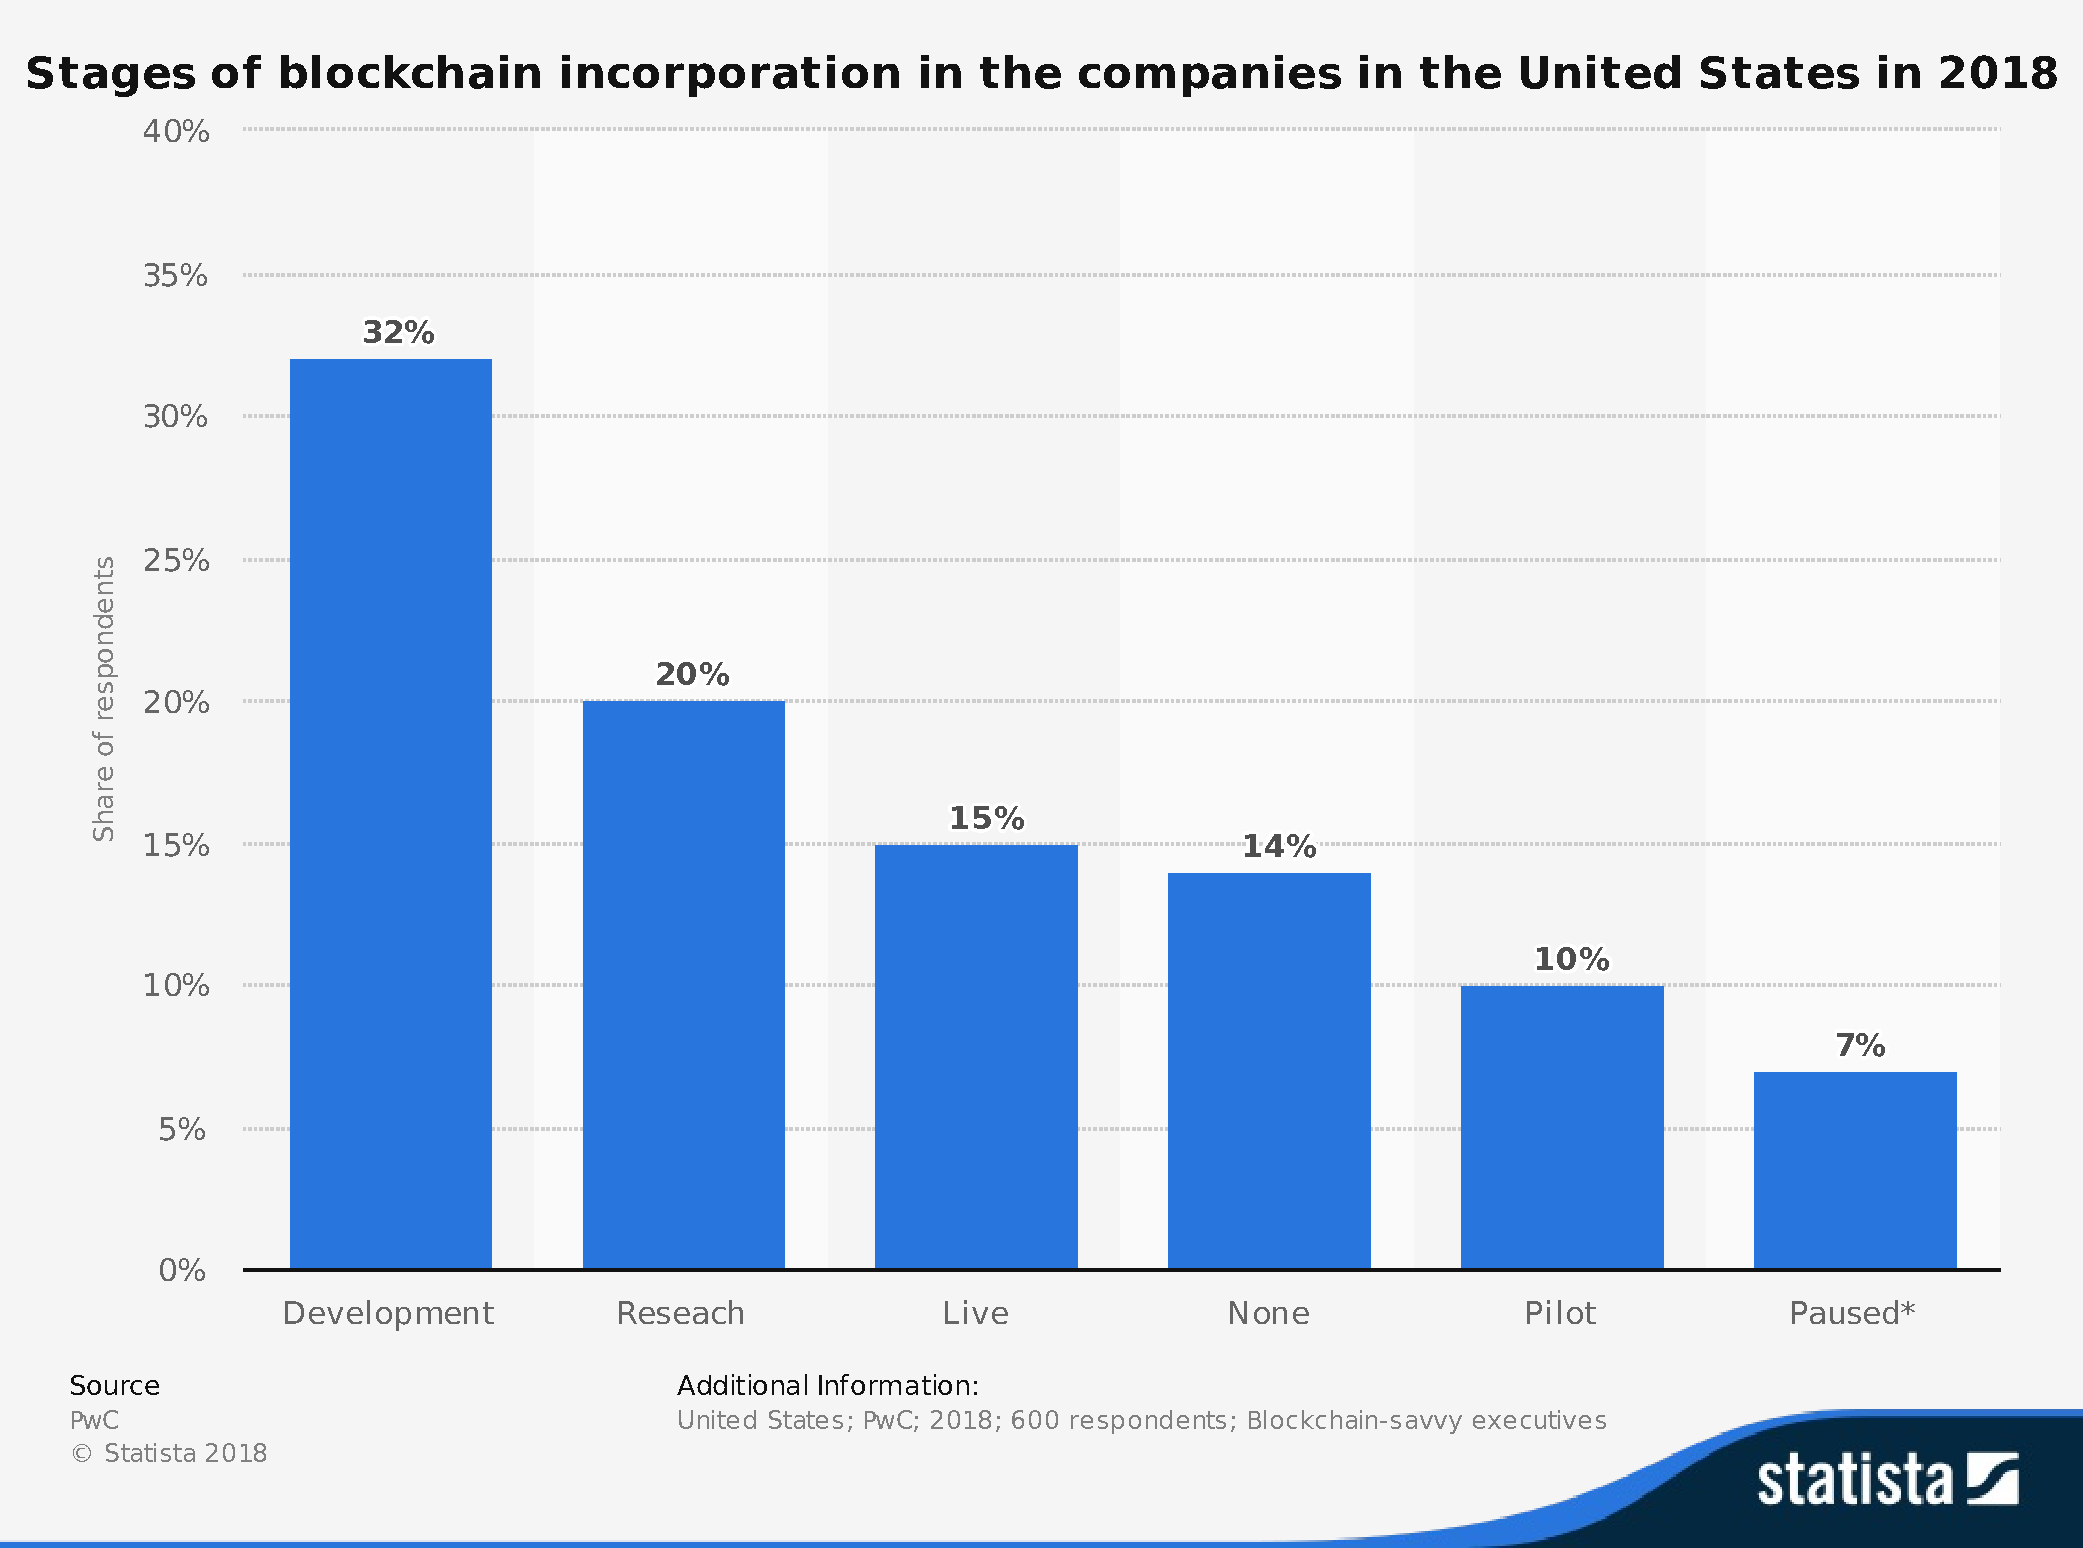
\includegraphics[width=1\linewidth]{images/chap_intro/stages-of-blockchain-incorporation.pdf}
		\caption{Livelli di adozione della blockchain nelle imprese U.S.
			\cite{stages-of-blockchain-incorporation}}
	\end{minipage}
\end{figure}

\subsection{L'evozione futura}
\begin{figure}[H]
	\centering
	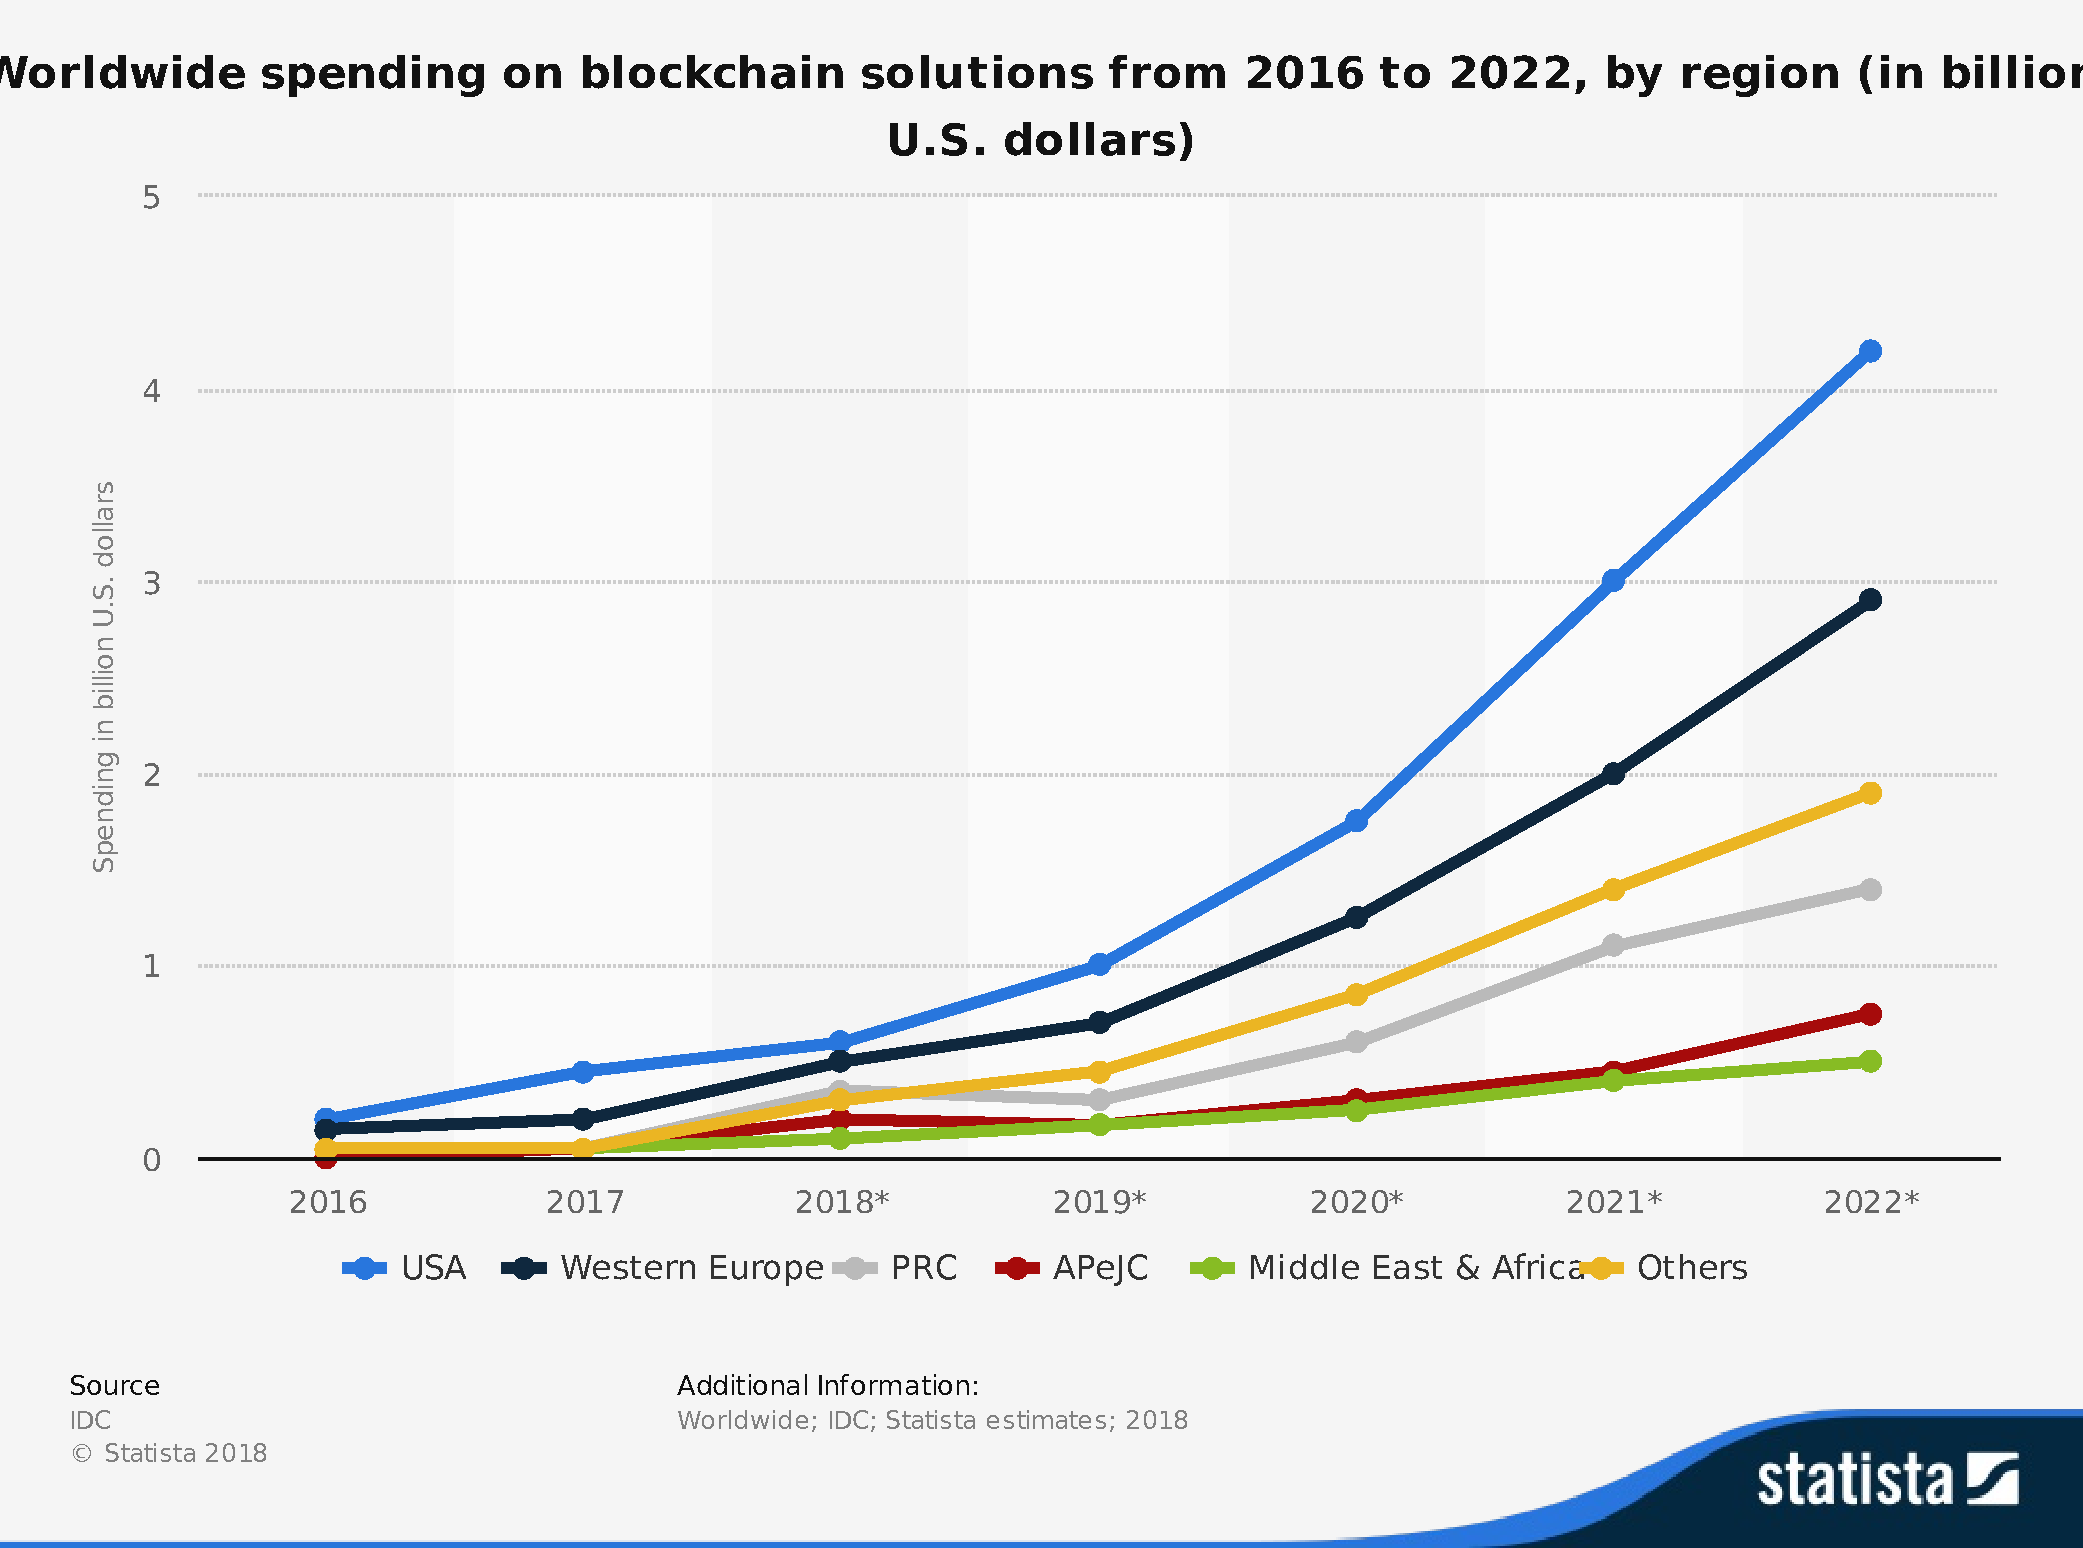
\includegraphics[width=.75\linewidth]{images/chap_intro/global-blockchain-solutions-spending.pdf}
	\caption{Spesa mondiale in soluzioni blockchain per regione (in miliardi di
		dollari U.S.) \cite{global-blockchain-solutions-spending}}
\end{figure}
\begin{figure}[H]
	\centering
	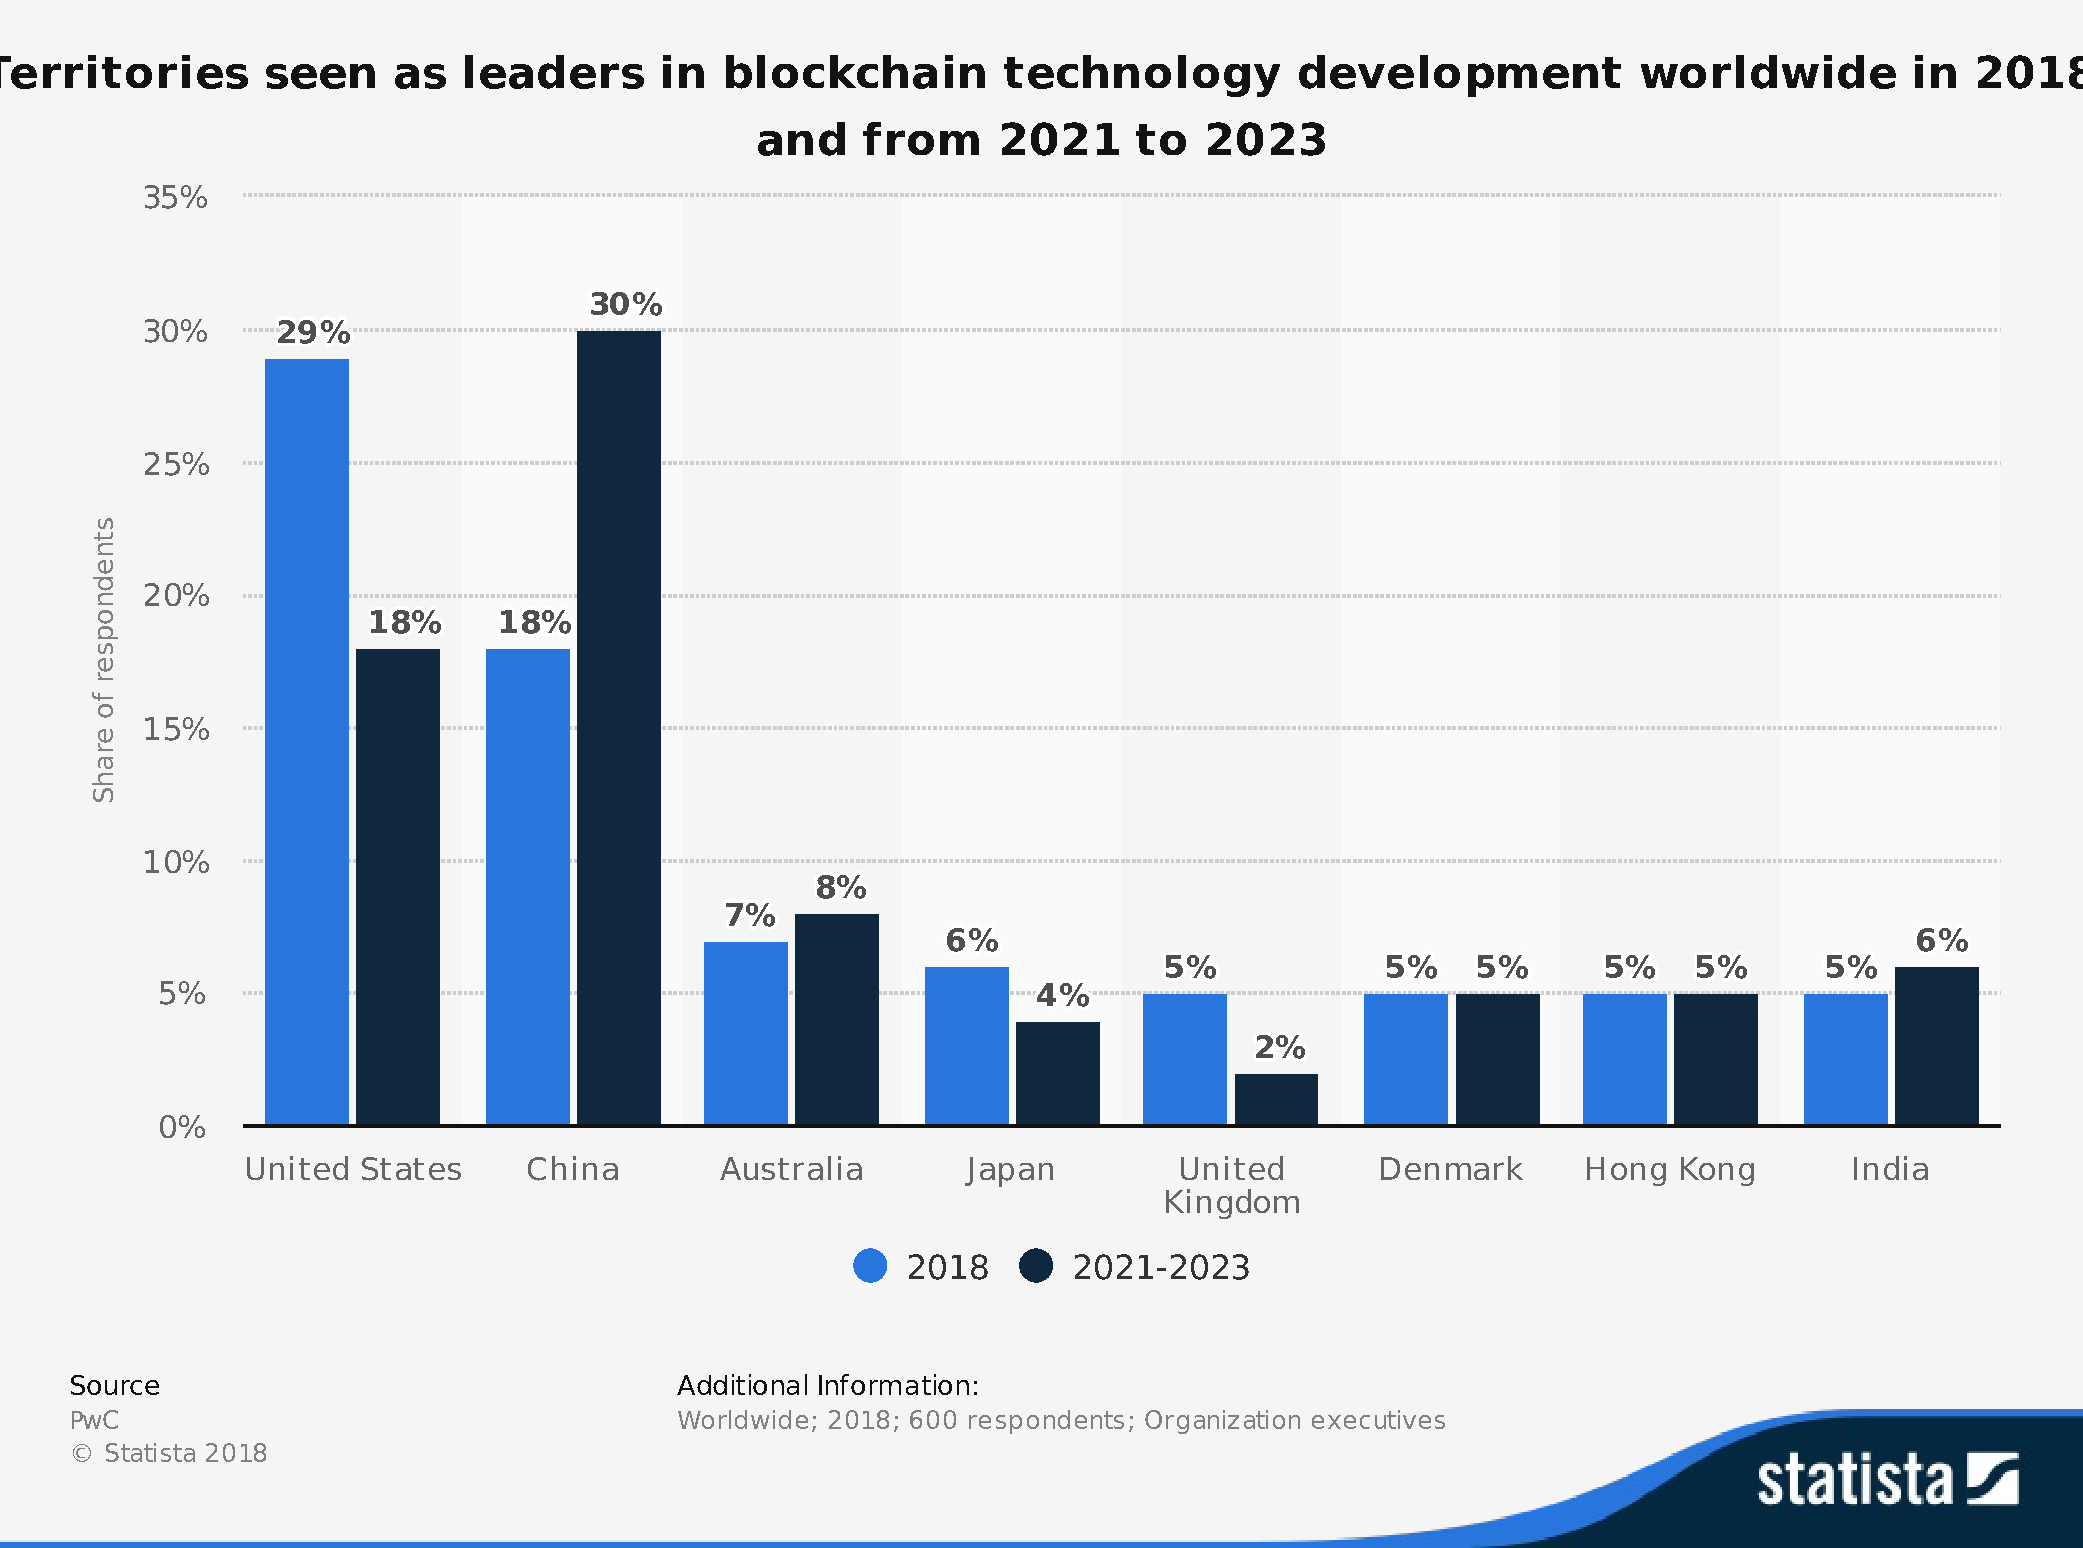
\includegraphics[width=.75\linewidth]{images/chap_intro/leading-territories-worldwide.pdf}
	\caption{
		\cite{leading-territories-worldwide}}
\end{figure}

\subsection{Le aspettative delle imprese}
\begin{figure}[H]
	\centering
	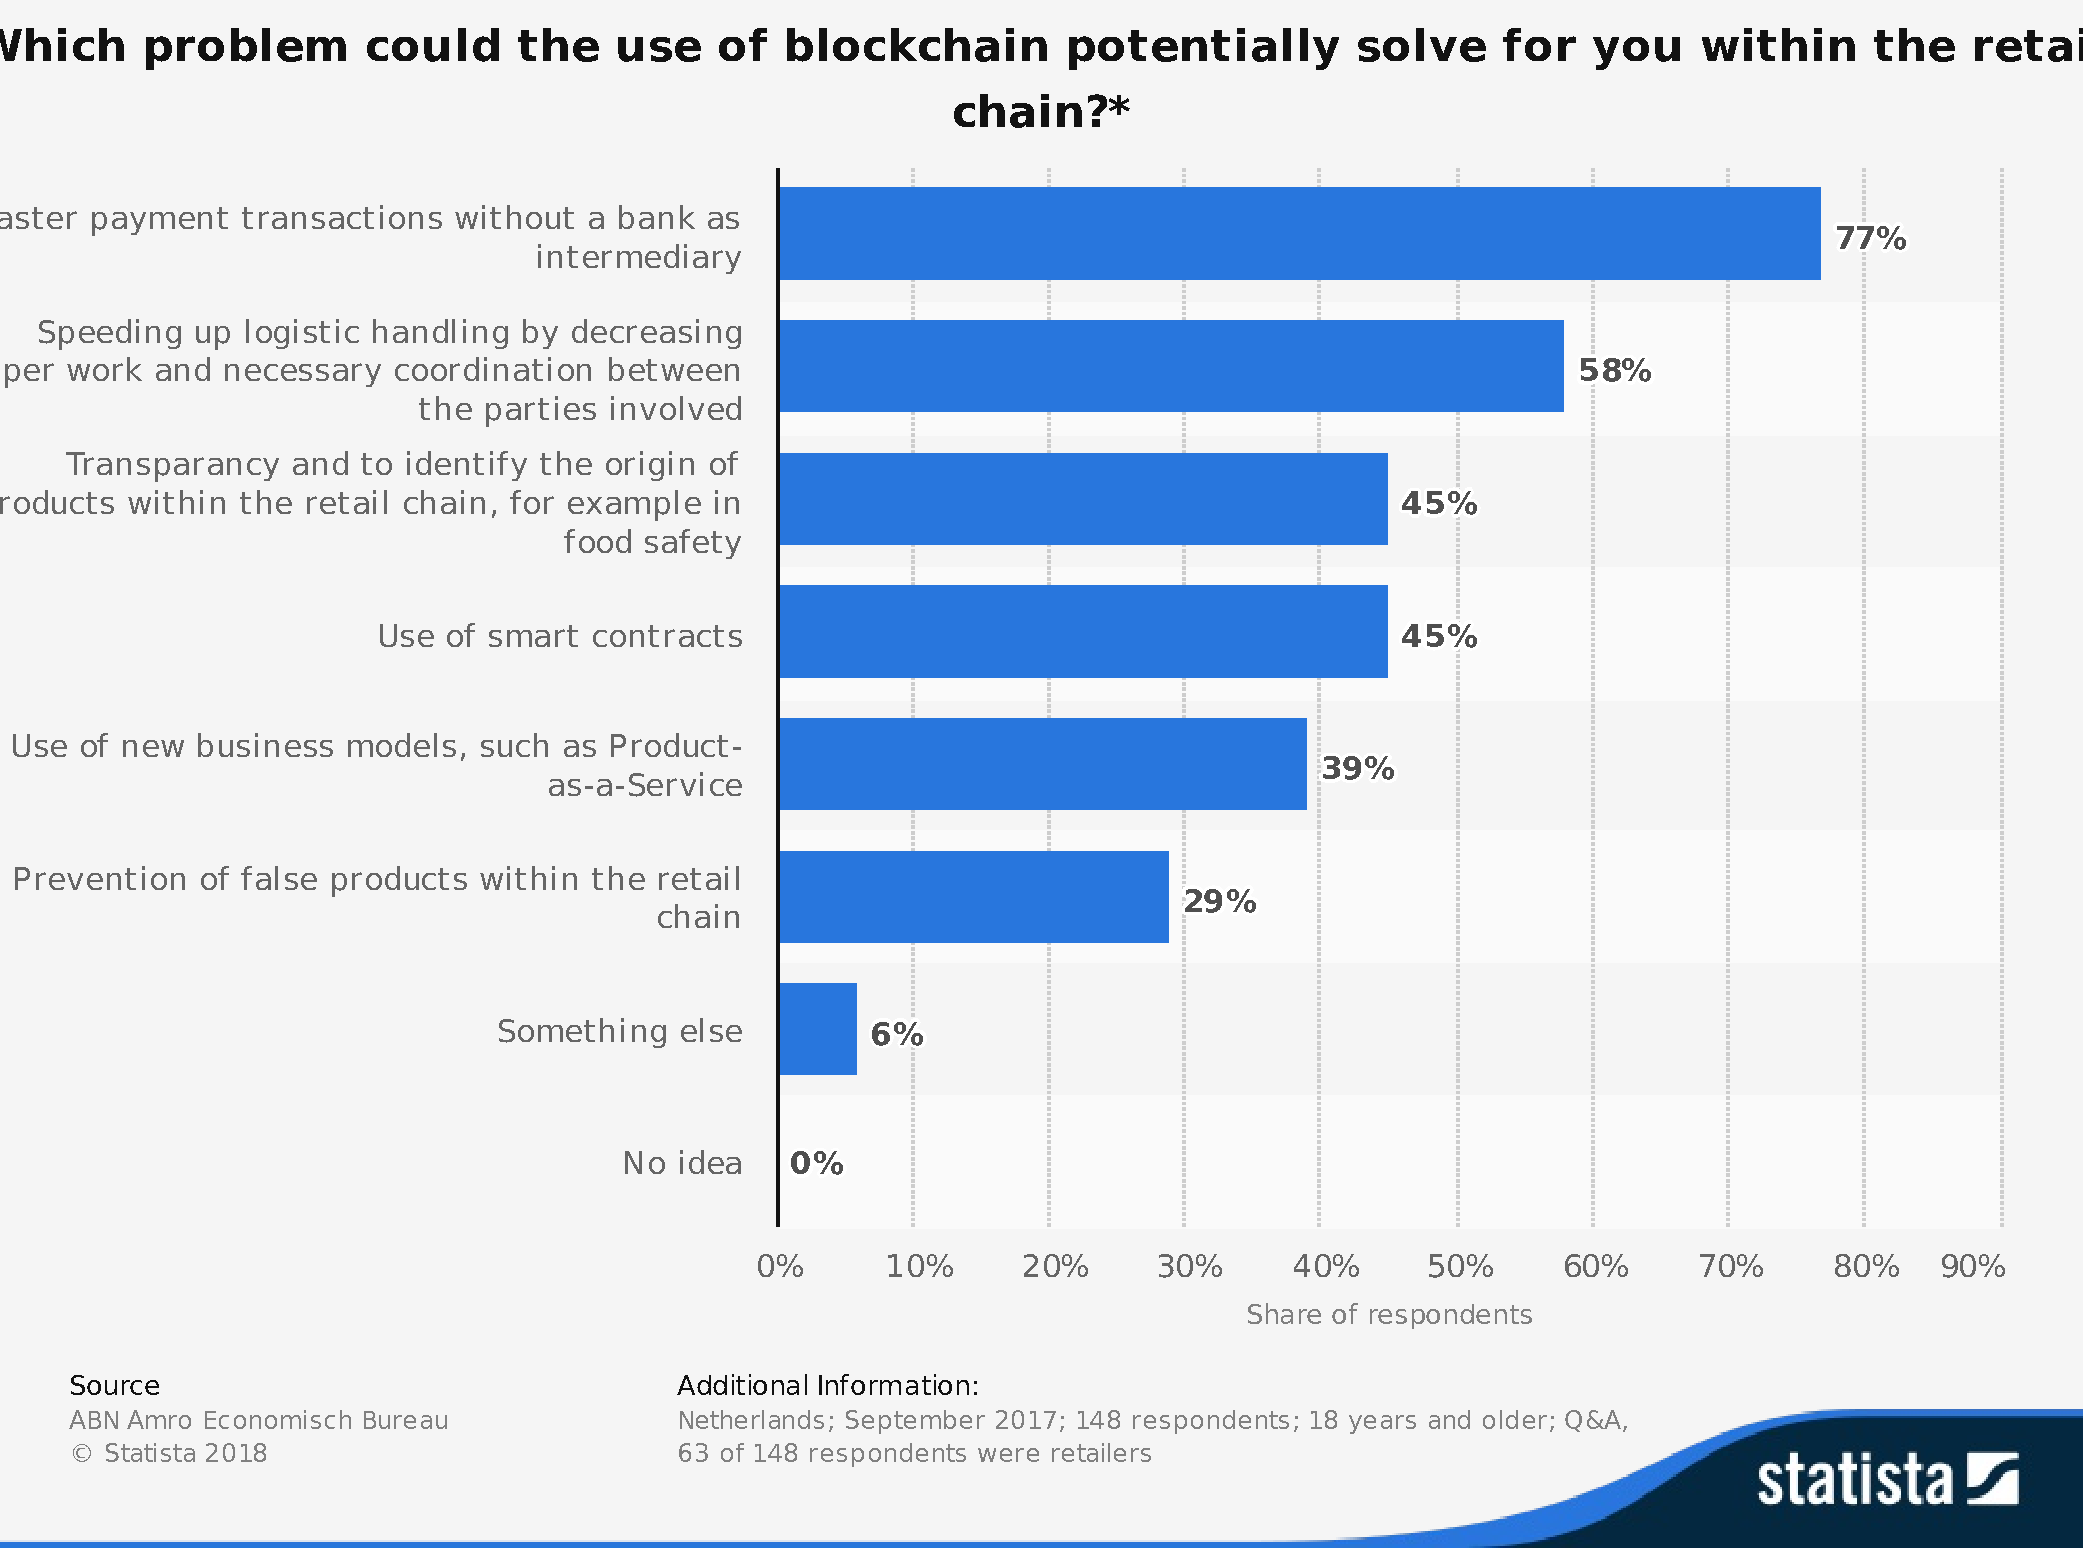
\includegraphics[width=.75\linewidth]{images/chap_intro/potential-blockchain-applications.pdf}
	\caption{Sondaggio: quale problema può potenzialmente risolvere l'uso della blockchain
		nella catena di commercio? \cite{potential-blockchain-applications}}
\end{figure}
\begin{figure}[H]
	\centering
	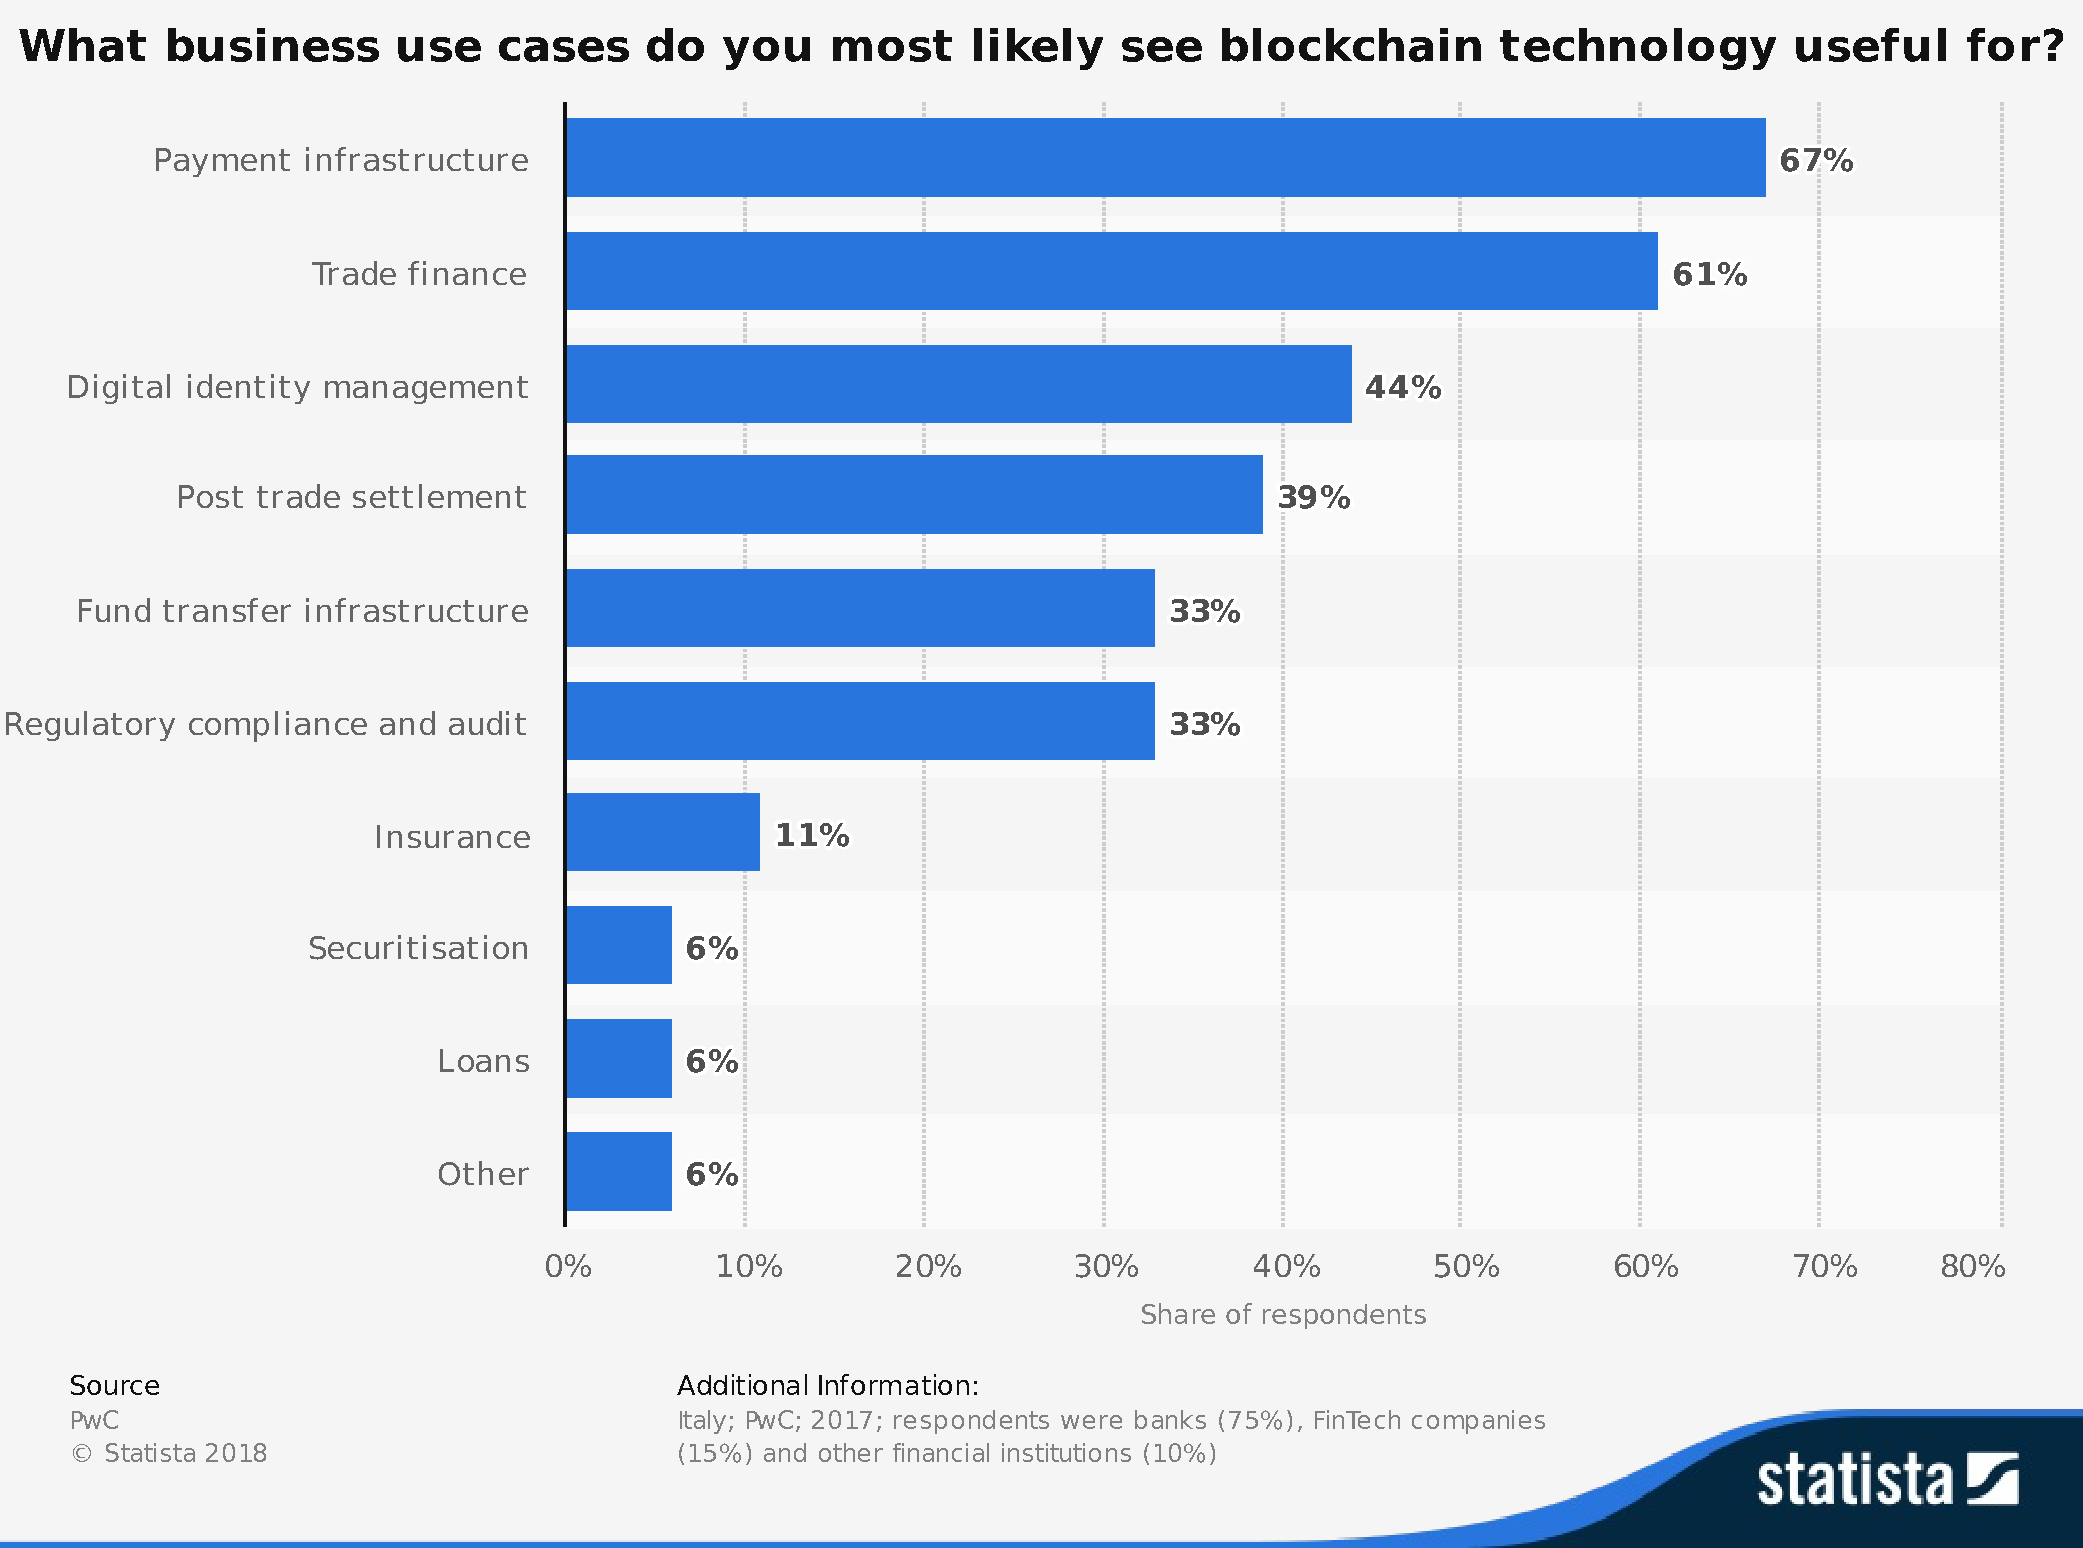
\includegraphics[width=.75\linewidth]{images/chap_intro/use-cases-among-businesses.pdf}
	\caption{Sondaggio: in quali caso d'uso di business la blockchain è utile?
		\cite{use-cases-among-businesses}}
\end{figure}
\begin{figure}[H]
	\centering
	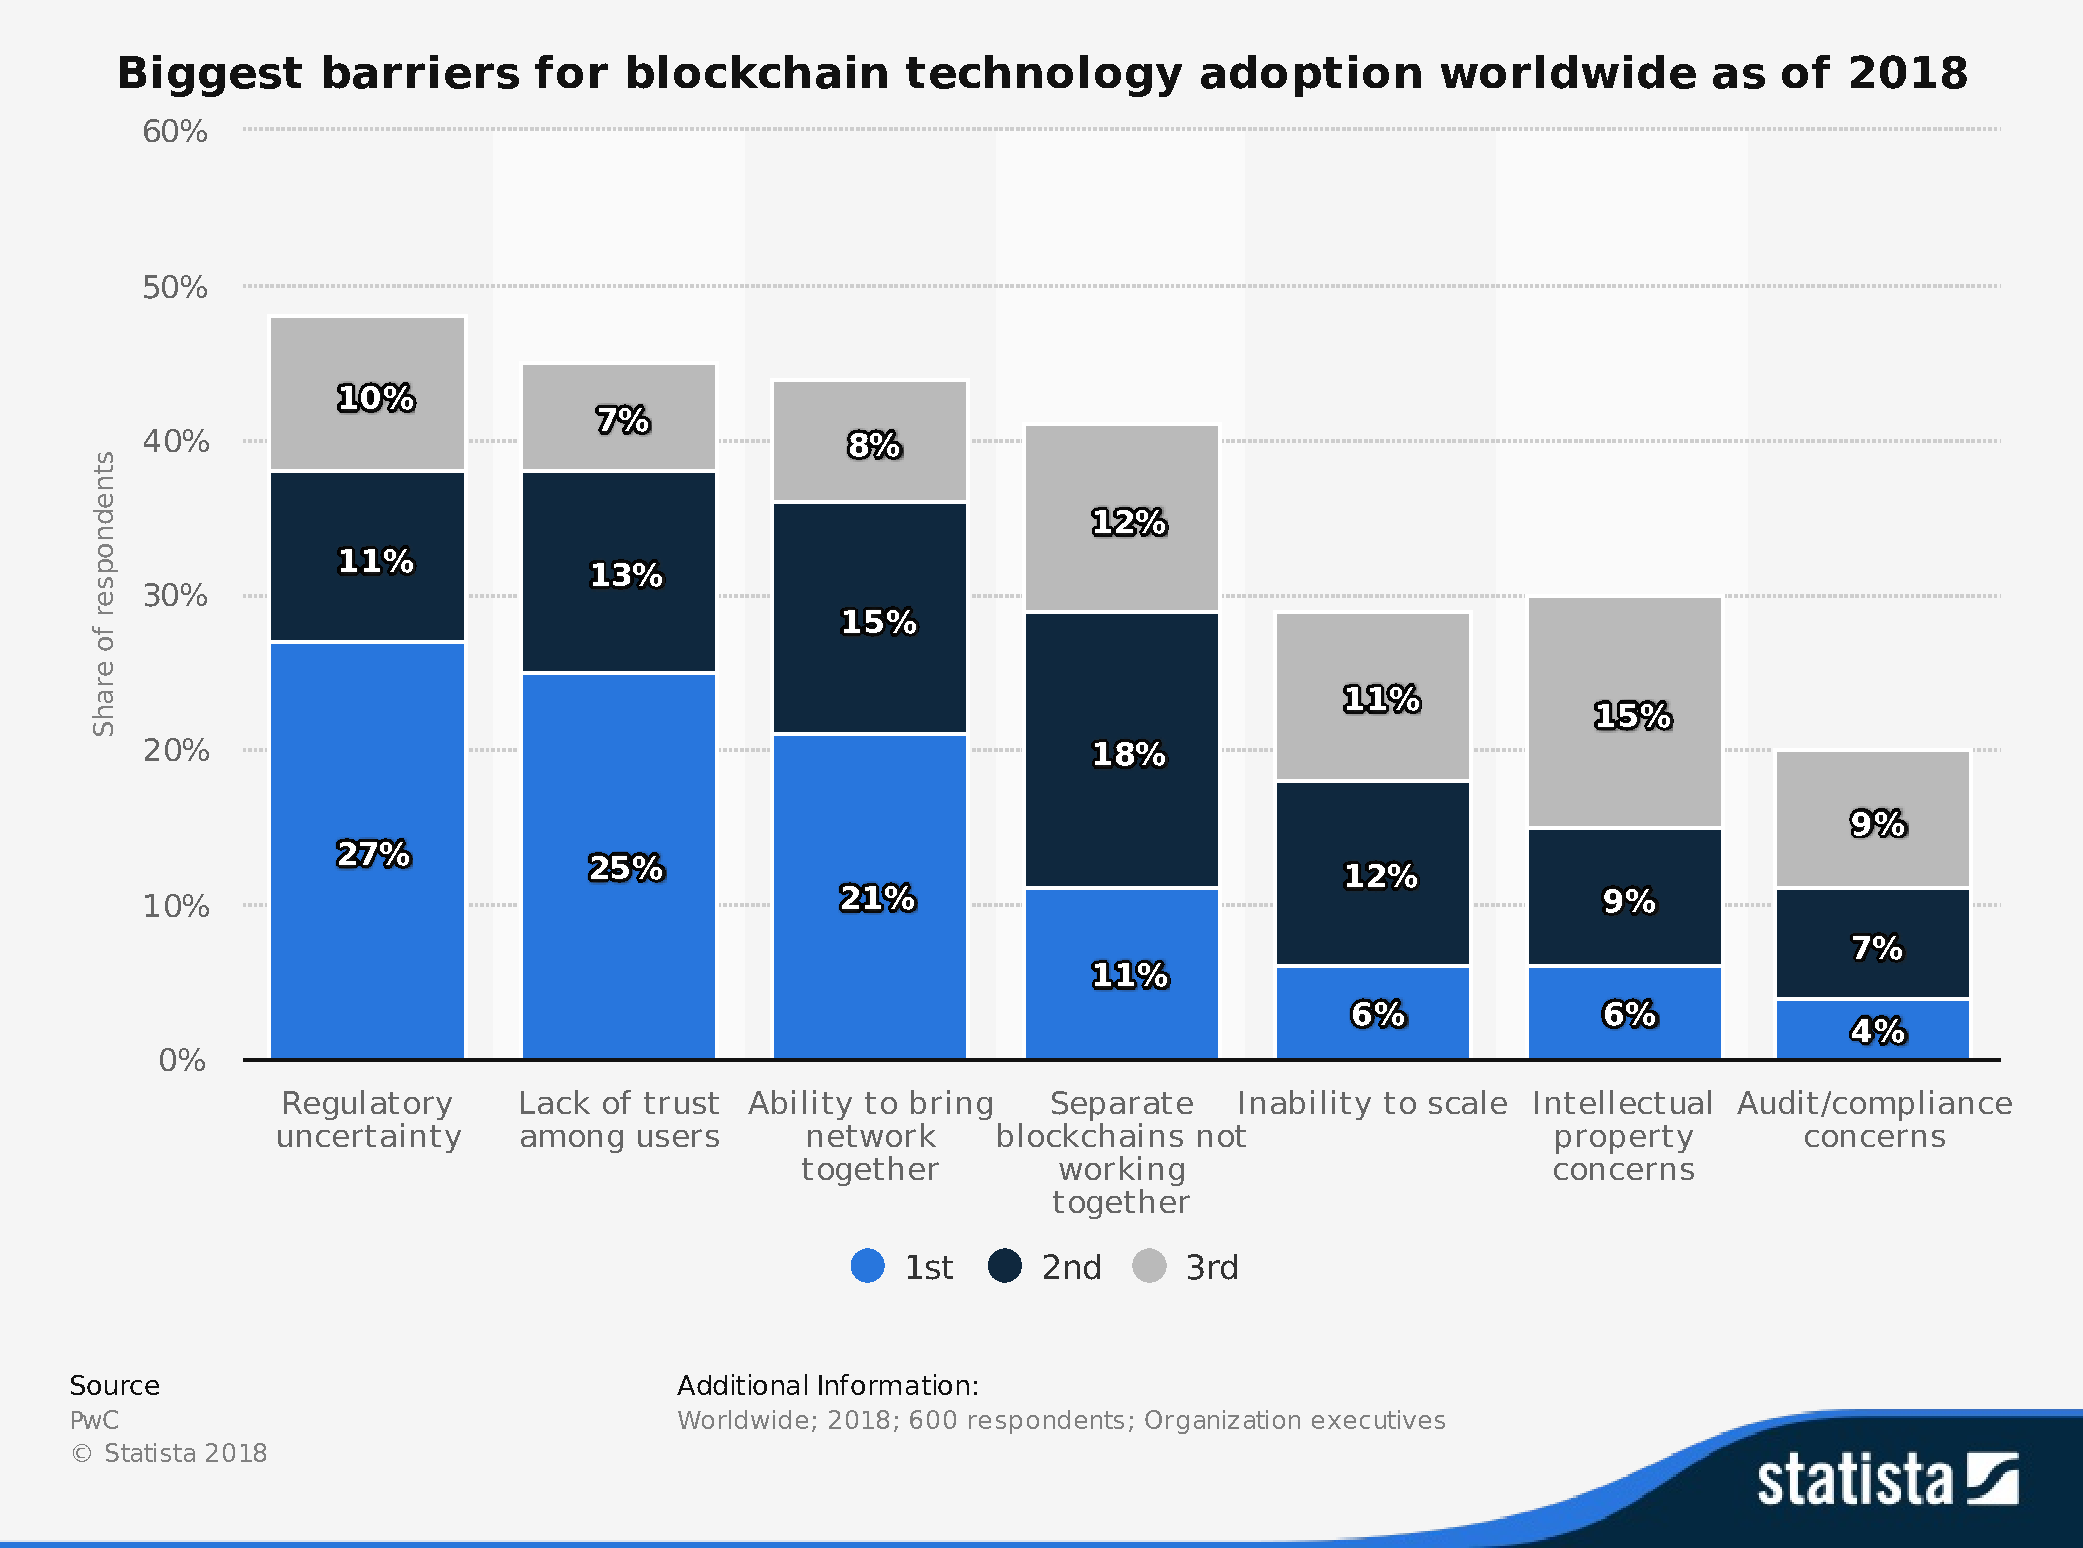
\includegraphics[width=.75\linewidth]{images/chap_intro/barriers-worldwide.pdf}
	\caption{
		\cite{barriers-worldwide}}
\end{figure}